\documentclass{beamer}
\mode<presentation>

\setbeamertemplate{navigation symbols}{}
\setbeamertemplate{theorems}[numbered]
\setbeamertemplate{items}[default]
\setbeamercovered{dynamic}
\setlength{\unitlength}{1cm}
\setbeamertemplate{footline}[frame number]

\usepackage{setspace}
\usepackage{amsmath,amssymb}
\usepackage{amsthm}
\usepackage{pgf,pgfarrows}
\usepackage[utf8]{inputenc}
% \usepackage[polish]{babel}
\usepackage{polski}
\usepackage{graphics}
\usepackage{tikz}
\usepackage[ruled]{algorithm}
\usepackage{algpseudocode}
\usepackage{scalefnt}
\usepackage{array}
\usepackage{colortbl}
\usepackage{float}
\usepackage{wrapfig}

\usetikzlibrary{arrows,automata,snakes}
\usetheme{Frankfurt}
\usecolortheme{seahorse} %crane
\useinnertheme{circles}


\newtheorem*{lemat}{Lemat}
\newtheorem{twierdzenie}{Twierdzenie}
\newcommand{\myitem}{\item[$\vartriangleright$]}
\newcommand{\nota}[1]{{\color{gray} \emph{#1}}}
\newcommand{\HarmonicN}[1]{H_{#1}}
\newcommand{\BALL}[2]{\mathbf{B}(#1,#2)}
\newcommand{\DISC}[2]{\mathbf{D}(#1,#2)}
\newcommand{\SPHERE}[2]{\mathbf{S}(#1,#2)}
\newcommand{\BigO}[1]{\mathcal{O}\left(#1\right)}
\newcommand{\BigTh}[1]{\Theta\left(#1\right)}
\newcommand{\slfrac}[2]{\left.#1\middle/#2\right.}
\newcommand{\PR}[1]{\mathrm{Pr}\left[#1\right]}
\newcommand{\E}[1]{\mathbb{E}\left[#1\right]}
\newcommand{\var}[1]{\mathbb{V}\mathrm{ar}\left[#1\right]}
\newcolumntype{C}{>{\centering\arraybackslash}p{0.5cm}}
\newcolumntype{Y}{>{\columncolor{blue!5}}C}

%\pgfpagesuselayout{4 on 1 with notes}[a4paper,border shrink=3mm]


\title{Bot do komputerowej gry wyścigowej}

\author{
	\textbf{Kamil Matejuk}
	\newline \newline
	Praca napisana pod kierunkiem \newline \textbf{dra Marcina Michalskiego}
}

\date{Styczeń 2022, Wrocław}


\begin{document}

\begin{frame}[plain]{}
	\titlepage
\end{frame}


\section{Wprowadzenie}
\begin{frame}{Cel i zakres pracy}

	\begin{itemize}
		\myitem Stworzenie gry wyścigowej 3D
		\myitem Stworzenie bota do gry
		\myitem Dokładniejsze poznanie silnika Unity, C\# oraz teorii Reinforcement Learning
	\end{itemize}

\end{frame}

\begin{frame}{Wybór środowiska}

	\begin{itemize}
		\myitem Darmowy silnik do tworzenia gier 3D
		\myitem Wsparcie dla wielu platform (PC, mobile, VR, etc)
		\myitem Jedno z najpopularnijszych rozwiązań na rynku (poza Unreal\textregistered)
		\myitem Niższa bariera wejścia niż Unreal\textregistered
	\end{itemize}

	\vspace{2cm}
	{\hspace*{5cm}\includegraphics[width=5cm]{figures/Unity_logo.png}}

\end{frame}


\section{Stworzenie gry}
\begin{frame}{Cel gry}

	\begin{itemize}
		\myitem Środowisko testowe dla bota
		\myitem Generator losowych terenów
		\myitem Gra single/multiplayer
	\end{itemize}

	\begin{figure}[!htb]
		\minipage{0.5\textwidth}
			\centering
			\includegraphics[height=3cm]{figures/terrains_2.png}
		\endminipage\hfill
		\minipage{0.5\textwidth}
			\centering
			\includegraphics[height=3cm]{figures/terrains_1.png}
		\endminipage
		\end{figure}

\end{frame}

\begin{frame}{Pętla}

	% \begin{itemize}
	% 	\myitem Wybór losowych punktów
	% 	\myitem Posortowanie punktów zgodnie z ruchem wskazówek zegara
	% 	\myitem Wybranie dodatkowych punktów kontrolnych
	% 	\myitem Połączenie punktów z wykorzystaniem krzywej Bezier 3 stopnia
	% \end{itemize}
	
	\includegraphics[width=\linewidth]{figures/loop_creation.png}

	% \vspace{2cm}
	\includegraphics[width=\linewidth]{figures/terrain_creation_1_2.png}

\end{frame}

\begin{frame}{Teren}

	\algrenewcommand\algorithmicrequire{\underline{\textsc{height(x, y)}}}
	\texttt{
	\begin{algorithmic}[1]
		\Require
		\Statex x $\gets$ (x + offset) * scale
		\Statex y $\gets$ (y + offset) * scale
		\Statex r1 $\gets$ detailsMain * Mathf.PerlinNoise(x/2, y/2)
		\Statex r2 $\gets$ detailsMinor * Mathf.PerlinNoise(x, z)
		\Statex r3 $\gets$ detailsTiny * Mathf.PerlinNoise(x*2, z*2)
		\Statex \Return r1 + r2 + r3
	\end{algorithmic}}

	\vspace{1cm}
	\includegraphics[width=\linewidth]{figures/terrain_creation_2_2.png}

\end{frame}

\begin{frame}[fragile]{Tekstury}

	\algrenewcommand\algorithmicrequire{\underline{\textsc{}}}
	\texttt{
	\begin{algorithmic}[1]
		\Require
		\Statex texture (
			\Statex \hskip2em float height,
			\Statex \hskip2em Vector3 normal,
			\Statex \hskip2em float steepness,
			\Statex \hskip2em float distanceToRoad
		\Statex ) \{ ... \}
	\end{algorithmic}}

	\vspace{1cm}
	\includegraphics[width=\linewidth]{figures/terrain_creation_3_2.png}

\end{frame}

\begin{frame}{Obiekty}

	\begin{columns}

		\begin{column}{.55\hsize}
			\begin{itemize}
				\myitem Start / Meta
				\myitem Pojazdy
				\myitem Elementy otoczenia
			\end{itemize}
		\end{column}
		
		\begin{column}{.45\hsize}
			\includegraphics[width=\linewidth]{figures/terrain_gen_params.png}
		\end{column}

	\end{columns}

	\vspace{1.5cm}
	\includegraphics[width=\linewidth]{figures/terrain_creation_4_2.png}

\end{frame}


\section{Stworzenie bota}
\begin{frame}{Reinforcement learning}
	
	\begin{center}
		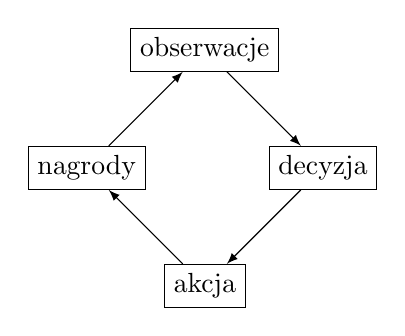
\begin{tikzpicture}
			\node[draw] at (0, 1.5) (1) {obserwacje};
			\node[draw] at (1.5, 0) (2) {decyzja};
			\node[draw] at (0, -1.5) (3) {akcja};
			\node[draw] at (-1.5, 0) (4) {nagrody};
			\draw [->,-latex] (1) to (2);
			\draw [->,-latex] (2) to (3);
			\draw [->,-latex] (3) to (4);
			\draw [->,-latex] (4) to (1);
		\end{tikzpicture}
	\end{center}
	
\end{frame}

\begin{frame}{Technologie}

	\begin{columns}

		\begin{column}{.4\hsize}
			\textbf{Unity MLAgents}
			\begin{itemize}
				\myitem Tensorflow
				\myitem Tensorboard
			\end{itemize}
		\end{column}
		
		\begin{column}{.6\hsize}
			\includegraphics[width=\linewidth]{figures/tensorboard.png}
		\end{column}

	\end{columns}

\end{frame}

\begin{frame}{Podjęcie akcji}
	
	\begin{columns}
		\begin{column}{.8\hsize}
			\textbf{ruch przód/tył oraz skręt kierownicy}
			\begin{itemize}
				\myitem wartości dyskretne $\{-1, 0, 1\}$
				\myitem wartości ciągłe $[-1, 1]$
			\end{itemize}
			
			\vspace{1cm}
			{\hspace*{2cm}\includegraphics[width=.8\linewidth]{figures/output_values_compare.png}}
		\end{column}

		\begin{column}{.2\hsize}
			\includegraphics[width=\linewidth]{figures/learning_loop_3.png}
			\vspace{5cm}
		\end{column}
	\end{columns}
	
\end{frame}

\begin{frame}{Ocena akcji}

	\begin{columns}
		\begin{column}{.65\hsize}
			\textbf{Po każdej akcji:}
			\begin{itemize}
				\myitem (0.3 - distanceToRoadCenter) * 0.01
				\myitem (distanceTraveledInFrame - 0.1) * 0.1
				\myitem (0.07 - abs(angleToTangent)) * 0.1
			\end{itemize}
			\vspace{5cm}
		\end{column}
		
		\begin{column}{.5\hsize}
			{\hspace*{.6\linewidth}\includegraphics[width=.4\linewidth]{figures/learning_loop_4.png}}
			\vspace{7cm}
			\includegraphics[width=\linewidth]{figures/rewards.png}
		\end{column}
	\end{columns}
	
\end{frame}

\begin{frame}{Ocena akcji}
	
	\begin{columns}
		\begin{column}{.5\hsize}
			\textbf{Przy kolizji:}
			\begin{itemize}
				\myitem z kolejnym checkpointem $+1$
				\myitem z innym checkpointem $-0.1$
				\myitem z krawędzią pola $-0.1$
			\end{itemize}
			\vspace{1cm}
			\textbf{Zakończenie epizodu po kolizji z krawędzą terenu/drogi}
			\vspace{3cm}
		\end{column}
		
		\begin{column}{.5\hsize}
			{\hspace*{.6\linewidth}\includegraphics[width=.4\linewidth]{figures/learning_loop_4.png}}
			\vspace{7cm}
			\includegraphics[width=\linewidth]{figures/checkpoints.png}
		\end{column}
	\end{columns}
	
\end{frame}

\begin{frame}{Wybór obserwacji}
	
	\begin{columns}
		\begin{column}{.8\hsize}
			\textbf{Obserwacje:}
			\begin{itemize}
				\myitem dane pobrane bezpośrednio z równania trasy
				\myitem dane odległości od krawędzi
				\myitem dane wizualne jednowymiarowe
				\myitem dane wizualne z kamery przedniej
				\myitem dane wizualne z kamery z lotu ptaka
			\end{itemize}
			\vspace{5mm}
		\end{column}
		
		\begin{column}{.2\hsize}
			\includegraphics[width=\linewidth]{figures/learning_loop_1.png}
			\vspace{15mm}
		\end{column}
	\end{columns}

	\begin{columns}
		\begin{column}{.3\hsize}
			\hspace*{3.9cm}
			\includegraphics[width=\linewidth]{figures/observations_2.png}
		\end{column}
	\end{columns}

	\begin{columns}
		\begin{column}{.3\hsize}
			\centering
			\includegraphics[width=\linewidth]{figures/observations_0.png}
		\end{column}
		\begin{column}{.3\hsize}
			\centering
			\includegraphics[width=\linewidth]{figures/observations_1.png}
		\end{column}
		\begin{column}{.3\hsize}
			\centering
			\includegraphics[width=\linewidth]{figures/observations_3.png}
		\end{column}
	\end{columns}
	
\end{frame}


\section{Podsumowanie}
\begin{frame}{Wybór obserwacji}
	
	\textbf{Wyniki}
	\includegraphics[width=\linewidth]{figures/input_observations.png}
	
\end{frame}

\begin{frame}{Dalszy rozwój}

	\begin{itemize}
		\myitem Wytrenowanie bota na większej ilości terenów
		\myitem Wytworzenie gry na różne platformy (np mobilne) 
	\end{itemize}

\end{frame}


\begin{frame}{}
	\begin{center}
		\large{Dziękuję za uwagę.}
	\end{center}
\end{frame}

\end{document} 